

\title{Reconocimiento de Patrones\\Tarea 3}
\author{Dietrich Daroch \qquad Diego Peña\\
ddaroch@uc.cl \qquad ddpena@uc.cl\\
}




\maketitle
\begin{abstract}
\begin{quote}
Este informe describe el trabajo realizado para la tarea 3 de reconocimiento de patrones, la cual consiste en medir la capacidad de los descriptores SIFT en conjunto con un clasificador VLAD de poder reconocer puntos de interés en imágenes y clasificar similares en base a coincidencias.
\end{quote}
\end{abstract}



% Introducción
% ============
%  Describe el problema a resolver, discutiendo aplicaciones relevantes al problema.
\section{Introducción}
\noindent El método de extracción de características \emph{Bag of Words} es altamente utilizado para describir texto. Éste método tiene un análogo visual (aún más general, \emph{Bag of Features}) en donde las ``palabras'' son \emph{patches} que pueden aparecer o no en una imagen.
Esas palabras ya no se pueden encontrar en un diccionario visual porque simplemente no hay. Se debe aprender las palabras útiles a partir de imágenes. Ese aprendizaje podría ser hecho usando rectángulos aleatorios de imágenes, pero no deberíamos esperar que sea muy bueno, sería como tomar substrings aleatorios de un libro y pensar que son palabras.
Para identificar las porciones importantes ya no basta mirar es espaciado de caracteres, se necesita identificar las porciones importantes de la imagen.
Para lograr identificar los lugares importantes en imágenes su usa descriptores que buscan dónde está la información valiosa (bordes). SIFT es uno de estos descriptores, tiene como objetivo ignorar diferencias no relevantes para la visión, como rotaciones y cambios de luminosidad.

Sin embargo, para datasets grandes con alto número de puntos de interés el poder de \emph{Bag of Features} disminuye y aumenta en gasto computacional. Es aqui donde VLAD (Vector of Locally Assigned Descriptors) supera a BoF en cuanto a poder de proceso al enfocar su clasificador en base a descriptores locales de la imagen de alto nivel, relacionando los datos más caracteristicos de dos imágenes a una comparación de distancia vectorial simple.

Como objetivo de este informe implementaremos y someteremos a \emph{test} la efectividad del método VLAD como extractor y clasificador e imágenes en base a características.






% Diseño e Implementación
% =======================
%  Aquí deben describir cómo resolvieron el problema, qué pasos siguieron y cómo implementaron la solución.
\section{Diseño e Implementación}


\subsection{Features}
Los siguientes filtros capturan algunas características de imágenes que intuitivamente son importantes a la hora de describir la forma, tarea esencial para poder reconocer dígitos.






% Implementación
% --------------
\subsection{Implementación}
%Usamos Matlab y vlfeat
El programa de reconocimiento fue desarrollado en entorno \emph{Matlab}, con ayuda de las librerías de acceso libre de \emph{vlfeat} \footnote{http://www.vlfeat.org/index.html}, la cual se especializa en implementar herramientas ppopulares de visión por computador especializadas en extracción de características y \emph{matching}.

Otras librerías ocupadas fueron \emph{rdir}, la cual permite acceso recursivo a directorios, dedicado al manejo de datasets grandes como con el cual trabajamos, y \emph{parfor}, que permitía mantener bajo vigilancia el progreso de varias secciones de trabajo pesado.



\subsection{\emph{Dataset}}
Como imágenes de prueba se utilizo el \emph{dataset} Oxford \footnote{http://www.robots.ox.ac.uk/~vgg/data/oxbuildings/}, provisto por el \emph{Visual Geometry Group} de la universidad de Oxford. Este set cuenta con 5063 imágenes de diversos \emph{landmarks} de la universidad de Oxford, clasificadas en 11 categorías, cada una perteneciendo a un sitio en específico fotografiado en distintas condiciones (\emph{distinta luz, multitudes, ángulo, entre otros}).

Via uso de descriptores entonces se busca poder reconcer a que categoría pertence cada foto del set de data (\emph{es decir, que landmark esta representada en la foto.}).

\subsection{\emph{Preparando las imágenes}}
El dataset fue preprocesado para lograr que las imágenes no exedieran los $640$ pixeles de ancho o alto. Esto fue realizado para disminuir la carga computacional al hacer la evaluación.
Pese a haber disminuido el tamaño de los datos, se espera que todavía sea suficiente ya que un humano aún puede reconocer imágenes de ese tamaño e incluso en imágenes más pequeñas.

Al inicio de la ejecución del programa se accede de manera recursiva a todo el set de datos, obteniendo una imagen tras otra. Información del \emph{path} de cada imagen se almacena, junto a otros datos, en un \emph{struct} especial a fin de obtener acceso más inmediato a ellos durante la implementación.

Como método de ahorro en computación, el conjunto de datos obtenidos de las imágenes son guardados en el archivo \emph{oxbuild.mat}, permitiendo acceso inmediato a él posteriormente y evitando cargar dos veces información que ya esta disponible.




\subsection{\emph{SIFT}}
Tras la obtención de imágenes se aplica un filtro \emph{grayscale} a la imágen para luego aplicarle el método \texttt{vl\_sift}.

Por cada imagen, este método devuelve dos tipos de descriptores:
\begin{itemize}
  \item \texttt{sift\_f}: devuelve un vector 4-dimensional con las caracteristcas de cada punto de interés dentro de la imagen: posición en coordenada X, posición en la coordenada Y, magnitud del vector descriptor y su orientación en radianes.
  \item \texttt{sift\_d}: Una matriz donde cada columna de 128 dimensiones contiene la descripción de una región en \texttt{sift\_f}
\end{itemize}

Ambos vectores se almacenan como campos en el \emph{struct} de cada imágen.

\begin{figure}[htb]
  \centering
  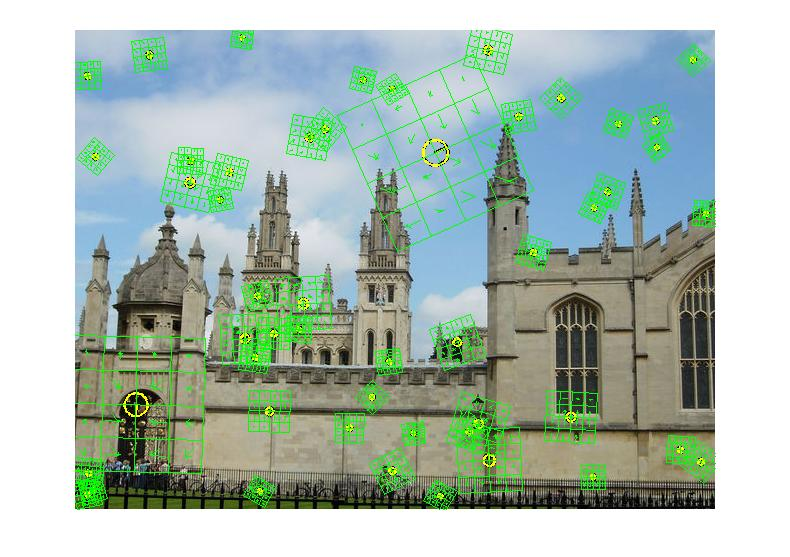
\includegraphics[width=\linewidth]{siftSample}
  \caption{Muestra de algunos de los features encontrados por SIFT en una de las imágenes del dataset. El rectángulo que muestra la rotación y escala está dividido en una grilla de 4x4 y cada celda tiene información del gradiente local.}
  \label{fig:siftSample}
\end{figure}



\subsection{\emph{Query management}}
Tras la extracción de los descriptores SIFT se recupera el \emph{query data} requerido para medir la eficacia de clasificación. Se arma nuevamente un \emph{struct} conteniendo la información de la consulta.

A partir del set de archivos se procede a extraer por \emph{mathcing} entre los nombres de los \emph{path} los archivos correspondientes a las consultas del set imágenes a catalogar, dejando dos subconjutnos de imagenes correspondiento a las consultas y no consultas.



\subsection{\emph{K-Clustering y Quantization}}
Tras la obtención de descriptores SIFT se obtiene una muestra aleatoria de 100000 de los vectores 128-dimensionales \texttt{sift\_d}.

A partir de esta muestra, los datos se someten al método \texttt{vl\_kmeans}, obteniendo los centros bajo 64, 128 y 256 clusters, y con ello las  \emph{visual words} requeridas para el cálculo de los vectores VLAD.

Con los \emph{clusters} ya obtenidos, como método de \emph{quantization} se procedió a obtener \emph{nearest neighbors} usando el método \texttt{kd\_trees}, obteniendo los descriptores SIFT más cercanos a cada centro.



\subsection{\emph{VLAD}}
Bajo la implementación explicada en el paper \emph{Aggregating Local Image Descriptors into Compact Codes}\footnote{Jegou, H.; Perronnin, F.; Douze, M.; Sanchez, J.; Perez, P.; Schmid, C., "Aggregating Local Image Descriptors into Compact Codes", Pattern Analysis and Machine Intelligence, IEEE Transactions on, vol.34, no.9, pp.1704,1716, Sept. 2012.}, para el correcto entrenamiento de VLAD se requiere, además de los datos y los centros obtenidos por el \emph{k-clustering}, una matriz de asignación correspondiente a los centros más representativos por cada imagen respecto al cluster.

Con ambos datos se uso la función \texttt{vl\_vlad} para obtener el vector VLAD de la imágen, almacenandola como campo en el \emph{struct} correspondiente.



\subsection{\emph{Ranking de resultados}}
Habiendo obtenido los vectores de descripción VLAD, se obtiene del query las 55 imágenes para realizar consultas.
Una por una, se compara y almacena la distancia entre el vector VLAD de la imágen consulta con todas las imágenes \emph{non-query}, valor que se va almacenando en una matriz para posterior análisis de resultados. La comparación por distancia fue realizada bajo \emph{euclidean} y \emph{hellinger distance}.








% Evaluación Experimental
% =======================
%  Describir los experimentos realizados, es importante mencionar los datasets que utilizaron, deben también discutir detalladamente los resultados obtenidos.
\section{Evaluación de resultados}

\subsection{Dataset}
Para la evaluación usamos el dataset \emph{Oxford Buildings}. Este dataset tiene $5063$ imágenes de edificios de la universidad. Para estas imágenes hay definidas $55$ consultas, para las cuales se espera recuperar un conjunto de imágenes de algún edificio en particular. Cada edificio tiene $5$ consultas asociadas.

\begin{figure}[htb]
  \centering
  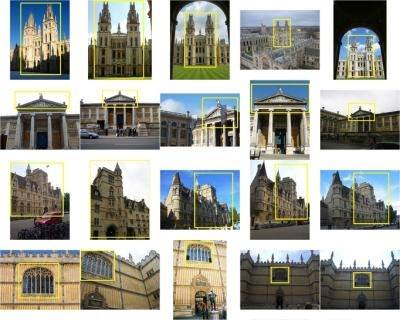
\includegraphics[width=.7\linewidth]{dataset}
  \caption{Muestra del dataset Oxford Buildings más puntos de interés}
  \label{fig:dataset}
\end{figure}

\subsection{Datos de trabajo}
Para el entrenamiento de los descriptores y vectores VLAD del programa, el anterior set de datos se dividía en dos partes:
\begin{itemize}
  \item Entrenamiento SIFT y VLAD: $5008$ imágenes
  \item Consulta: $55$ imágenes
\end{itemize}

\paragraph{}
Cada Consulta tiene $4$ conjuntos de imágenes asociados:
\begin{itemize}
  \item \emph{good}: Una foto buena del edificio.
  \item \emph{ok}: Una foto un poco ocluída, pero al menos el 25\% del edificio se puede ver.
  \item \emph{junk}: El edificio aparece, pero se puede apreciar menos del 25\%.
  \item \emph{bad}: El edificio no aparece.
\end{itemize}


\subsection{Descriptores SIFT}
La implementación del metodo \texttt{vl\_sift} extrajo con buenos resultados los puntos de interés, enfocandose en esquinas en especial, distribución de patrones en arquitectura y ambiente sin gran efecto causado por cambios de luz o presencia de objetos externos. Los edificios de interés fueron correctamente identificados.
\begin{figure}[htb]
  \centering
  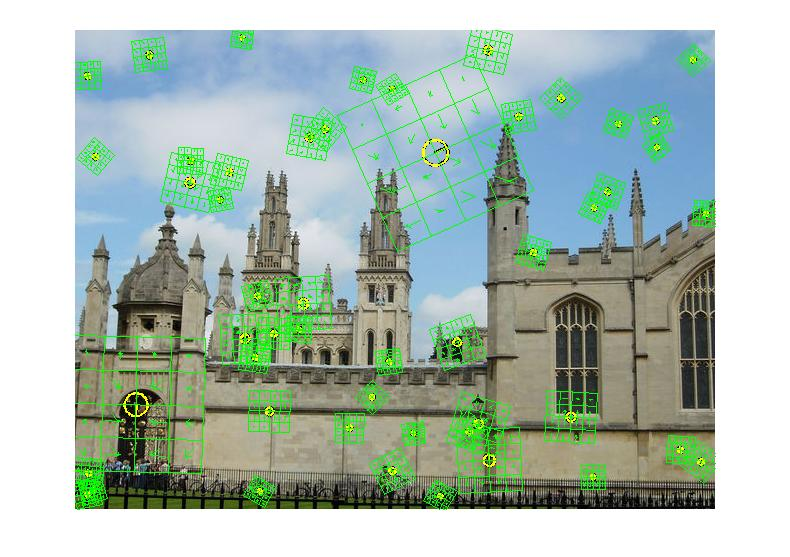
\includegraphics[width=.9\linewidth]{siftSample}
  \caption{Muestra de descriptores SIFT en imágen}
  \label{fig:siftSample}
\end{figure}


\subsection{Resultados y ranking por VLAD}

Al calcular la distancia de las foto de la consulta con el resto de la base de datos se induce un orden de relevancia.
En esa lista esperamos encontrar a las fotos clasificadas como \emph{good} para la consulta en las primeras posiciones.

Esto no ocurrió así, en algunas consultas obtuvimos 5 fotos dentro de las 100 primeras propuestas. Lo cual si bien reduce en gran parte el espacio de búsqueda, no lo hace suficientemente como nos gustaría.

Logramos obtener una lista con las posiciones que ocupaban las fotos esperadas en el \emph{ranking}, pero no pudimos construir el gráfico esperado con \texttt{vl\_pr}, ya que lo que obtuvimos en el gráfico contradecía fuertemente a lo que sabíamos que había pasado.

% mandamos??
% adjuntale un link al repo de github para que vea que intentamos hacer bien la wea xd
% si, mandemos no mas
%pero hay que mandarle el codigo tambien no?
%yap, makes sens
% mandale el zip de github https://github.com/dgopena/patrones-T3/archive/master.zip


% Conclusiones
% ============
%  Describir las conclusiones obtenidas luego de desarrollar la tarea o el proyecto.

\subsection{Conclusión}

% pero los resultados son malos o no?

De nuestros resultados podemos concluir que VLAD en conjunto con SIFT son un medio muy eficiente para clasificar y extraer características de grandes datasets de imágenes.

Con mayores niveles de clustering la fiabilidad de los resultados aumentan junto a un pequeño aumento en la exigencia de procesamiento. Gran aporte a la velocidad de clasificación es la reducción de descriptores a un vector representativo de cada imagen, pudiendo realizar la comparación entre miembros del \emph{dataset} de manera simple y rápida por medio de una diferencia vectorial entre los VLADs respectivos.

Sin embargo, la inmediatez de VLAD en entorno \emph{Matlab} se debe en gran parte a la capacidad de almacenar resultados, y estos ocupan mucho espacio dada la gran cantidad de datos que cada imagen contiene en conjunto por sus descriptores SIFT como su vector VLAD. En términos de uso de memoria entonces, este método no es óptimo.
